The purpose of this case is to test the calculation of loss curves and average loss for the contents of an asset. The replacement value of the contents for the asset used in this case is $5,000$. Table~\ref{tab:vf-ln-tax1-con} shows the mean loss ratios and corresponding coefficients of variation in the contents vulnerability function used in this test case. Apart from the change in the vulnerability function and value, the calculation procedure remains the same as described in Case~1d.

The loss curve calculated using the implementation of the calculator in Julia is compared with that produced by OpenQuake in Figure~\ref{fig:lc-ebr-2b}.

\begin{figure}[htbp]
\centering
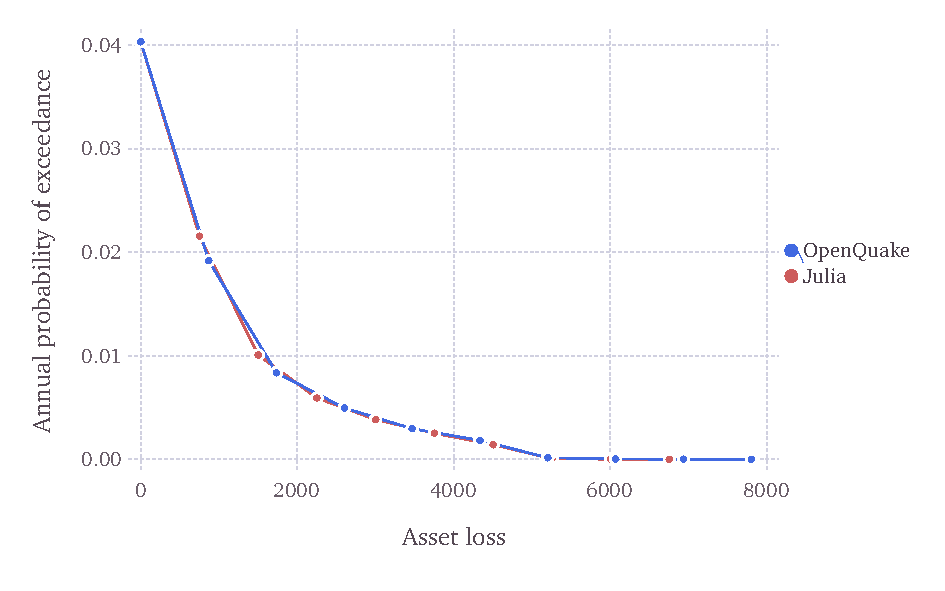
\includegraphics[width=12cm]{qareport/figures/fig-lc-ebr-2b}
\caption{Loss curve comparison for event based risk test case 2b}
\label{fig:lc-ebr-2b}
\end{figure}